%ब
\section{Experimental API}\label{s:implementation-API}

The experimental \ac{API} was designed generically in order to ensure that it
can be used by  applications to maintain dependencies within their keyspaces
irrespective of keyspace schemas or structures of column families.  However,
applications using this \ac{API} still have to supply  the list of referential
integrity constraints as these are not automatically deduced from their
implementation. Instead, the constraints have to be introduced according to the
solution as it is explained in detail in
Section~\ref{s:implementation-MDinSolutions}.

% Thus,   this \ac{API} is made adaptable to different keyspace schemas  that
% can be deployed in column-oriented key-value \acp{DBMS}.

This \ac{API} validates the referential integrity based on the metadata provided
for the application and its column families.   It  provides the implementation of
all the four solutions as well as the required components to successfully
maintain referential integrity in Cassandra.

The  class diagram of the \ac{API} is presented  in
 Figure~\ref{f:classDiagram} alongside with the  classes that belong to 
the University keyspace example.  The design of the \ac{API} follows the
\ac{ER} model and the main components are the entities, entity managers,  and
validation handlers,  all of which are described in the next sections.
 Notice that for the sake of clarity and brevity,   the class diagram only
 contains  the relevant  methods of the classes,  favoring a simpler
explanation of the functioning of the \ac{API}. 

\begin{figure}[h]  
	\centering
	%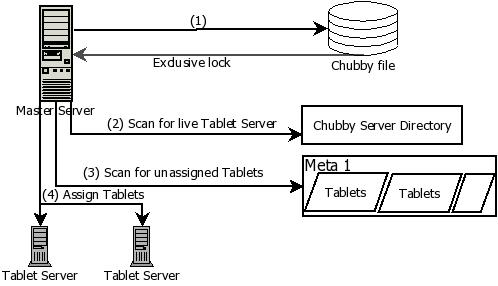
\includegraphics[width=5cm,    height=5cm]{.  /figure/random.  jpg}
	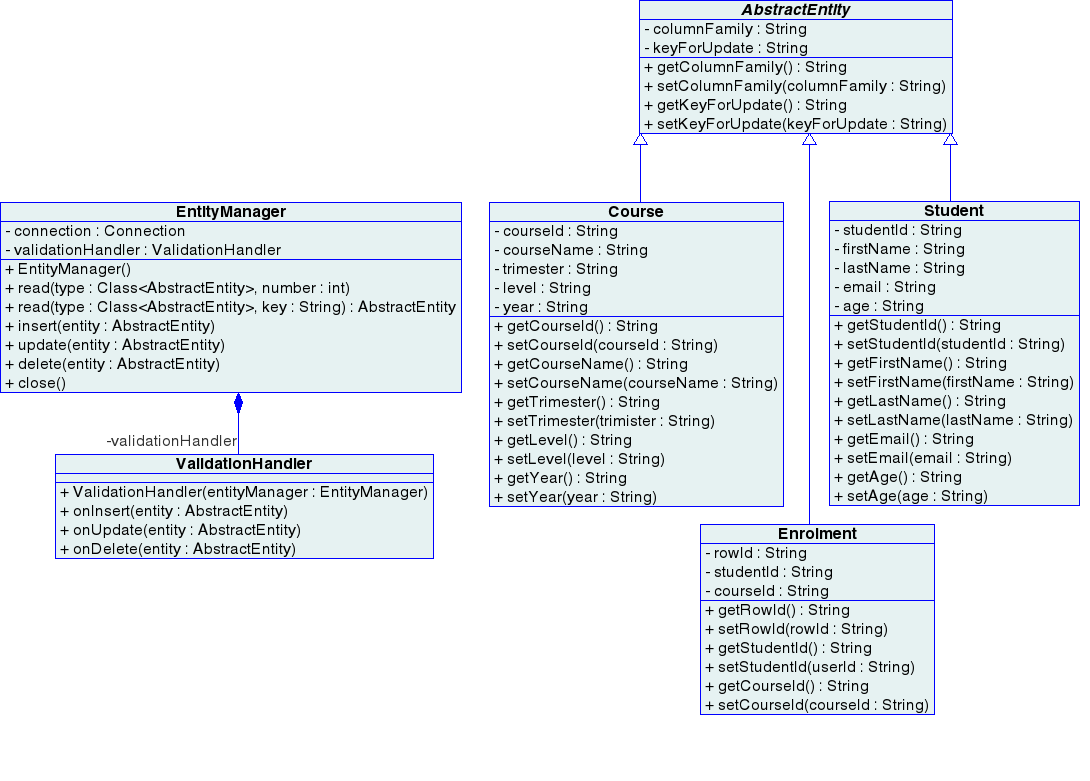
\includegraphics[width=\textwidth]{./figure/Solutions/FinalClassDiagram.png}
	\caption{Class Diagram for the \ac{API}}\label{f:classDiagram}
\end{figure}


	\subsection{Entities} 
	
	An \texttt{Entity} class contains attributes (with respective getters and
	setters) that map to columns within a specific column family.  As such,  the contents of a
	column family can be represented by a list of entity objects.  All entities in
	the \ac{API} extend from the class \texttt{Entity}  to
	aid the \ac{API} towards their management.  Particularly,  the attributes
	that \texttt{Entity} contains  are \texttt{columnFamily} which
	determines the column family to which the entity maps,  and 
	\texttt{keyForUpdate} which shall contain the new value in case the primary key
	of the entity is to be updated. 
	
	For example,   considering the University keyspace example,  \texttt{Enrolment} 
	is an entity class that  maps to the \texttt{Enrolment}  column family,  thus
	containing the attributes \texttt{RowId},  \texttt{CourseId} and
	\texttt{StudentId} which represent its respective columns.  As such,  an
	instance of \texttt{Enrolment} contains the values of one super column.  Likewise, 
	\texttt{Student} and \texttt{Course} are entity classes and their instances 
	map to   super columns in their respective column families. 
% 	For all the solutions in this \ac{API},   entities of the user applications are
% 	designed to extend the abstract class called \texttt{Entity},   which has
% 	information about the  methods for accessing and defining  entities.   For
% 	every column family,  applications derive a class from the
% 	\texttt{Entity} containing attributes. 
	Thus, the \ac{CRUD} operations that are performed on these entities  and are
	handled by the \texttt{EntityManager} class, explained next. 
		 
	\subsection{EntityManager} \label{ss:Implementation-API-EntityManager}

	The  \texttt{EntityManager} class implements  all
	the \ac{CRUD} operations to be performed on the entities.  In order to perform
	these operations,   the \texttt{EntityManager} interacts with the respective
	keyspace the entity belongs.  Moreover,  it ensures to trigger the   referential
	integrity validation process whenever a \ac{CRUD} operation requires it. The
	\texttt{EntityManager} contains an instance of \texttt{ValidationHandler} which
	ensures the validations.
	
	The \texttt{EntityManager},  before performing any operation,  requires a
	connection to the keyspace.  This connection is established using a third-party
	\ac{API} named Hector~\citep{hector}.  Hector  encapsulates the driver-level
	interface provided by Cassandra (known as Thrift) and simplifies the interaction
	with it.  Regarding the \ac{CRUD} operations,  Hector provides  a
	\texttt{Mutator} object which encapsulates the necessary procedures to perform
	such operations and to interact with the Cassandra cluster.
	 
	 Notice that  the \texttt{EntityManager} is able to generically deal with any
	 entity that derives from the \texttt{Entity} class.  It does so by using
	 reflection,  a Java  feature that is able to perform an introspection of an
	 object in runtime and retrieve its attributes and methods. 
% 	  to detect the
% 	 attributes of an object and generically invoking the getters and setters of the entities.  
	 Thus,  the  \texttt{EntityManager} is able to perform all \ac{CRUD} operations
	 on any entity by generically invoking its getter and setter methods.
	 
	 
	
% 	Hector is a high
% 	 level client that wraps the driver-level interface of Cassandra called Thrift. 
% 	 Hector  provides some features that  Thrift does not,  for example,  
% 	 fail-over mechanisms and connection pooling (\todo{cite book}).   
	 % 	 While there
% 	 are other wrappers for Thrift,  Hector was  chosen as  it is one of the
% 	 earliest wrappers and  encapsulates the interaction with the Thrift \ac{API}
% 	 and makes it simpler to access a Cassandra cluster. 	
	
	
	
	
		\subsubsection{Create}
		The \texttt{create} (or \texttt{insert}) operation stores entities in their
		respective column families. This method is provided by the
		\texttt{EntityManager} and it manages to insert these entities into their
		resective  column families which are represented by the entity class.
		For example, all the student entities are inserted into the column family
		\texttt{Student} through the \texttt{EntityManager}.  
		
		The \texttt{insert} operation triggers a referential integrity validation
		whenever a child entity is  inserted in order to ensure that its parent entities
		exist.  The validation is performed by the \texttt{onInsert} method of
		\texttt{ValidationHandler},  which is explained later.  Finally, if the
		\texttt{ValidationHandler} allows it, the \texttt{EntityManager} passes the
		entity details  including row key and column family as
		parameters to the \texttt{addInsertion} method of the Hector \texttt{Mutator}
		object.
			
		\subsubsection{Read}
		The  \texttt{read} operation retrieves  entities from the column family mapped
		by the entity class.		
		This \ac{API} provides three methods for retrieving entities: \texttt{find},
		\texttt{query} and \texttt{read}. The \texttt{find} mehtod retrieves a single
		entity given its class and the value of its primary key. The \texttt{query}
		method retrieves a list of entities given a conditional expression on a
		column  name and a column value. The \texttt{read} method retrieves a list of
		entities representing the contents of the column family.
		
		Notice that, these  operations do not prompt any referential integrity
		validation since entities are only read and their state is not changed,  unlike
		in the other operations.

		
		
		\subsubsection{Update}\label{ss:update}
		The \texttt{update} operation merges  the existing contents of an entity  with
		new contents.   In other words,  the  values of the columns an entity represents
		are updated to new values and committed into the column families.
		
		The \texttt{EntityManager} provides the following three types of updates. 
		
		\begin{description}
			\item [Case A: Update Primary Key]  where the attribute
			\texttt{keyForUpdate} is used to indicate the change in the primary key.
			Before the primary key is updated, and there are child dependencies referencing
			the primary key,  the following steps are performed to complete the
			\texttt{update} operation.
		% In order to do so,  the \texttt{EntityManager} passes the entity to the
		% \texttt{ValidationHandler}  to check for referential integrity,  retrieves the
		% list of child entities that depend on its primary key,  deletes dependencies
		% and the entity,   and update the dependencies Following this,  the steps that
		% are performed are :
\todo{FIX}
			\begin{enumerate}
			  
			  
			\item Check with the \texttt{ValidationHandler} if the entity can be updated.
		
			
			\item Set the primary key of the entity to the \texttt{keyForUpdate} value. 
			
			\item Perform an \texttt{insert} of the entity with the new primary key.
			
			\item Retrieve the list of any child entities that depend on the old primary key
			of the entity.

			\item Update the foreign keys of the list of child entities to match the value
			of the new primary key of the entity.
			
			\item Perform a \texttt{delete} operation on the old entity.
		\item

			\end{enumerate}
		
% 		In all the solutions,   an \texttt{Update} operation triggers a referential
% 		 integrity validation whenever any primary or foreign keys of any entities are
% 		updated. 
% 		The validations are performed by the \texttt{onUpdate} method of the
% 		\texttt{ValidationHandler}. 
			If the update is not a cascaded one, the child entities are not updated to
			the new primary keys. This is explained in Section~\ref{} Notice that such a
			procedure is used to circumvent the restriction of Cassandra to change a primary key.  Once a record has been
			inserted into the column family,  the primary key cannot  be changed.  This is
			known as a tombstone delete,  which prevents deleting a primary key or
			changing it. 
		
		
		
			\item [Case B: Update  Foreign Key]  where  the \texttt{ValidationHandler}
			is used to check if the foreign keys can be updated and
			the respective getter and setter methods of the entity are used to perform the
			changes. 
			
			\item [Case C: Update Attributes]  where a normal update takes place as long as
			the attributes  are not keys or referenced anywhere.
			
		\end{description}
		
		
% 		one in which ,   another in which the foriegn keys are changed
% 		and lastly the one in which attributes that are not keys or referenced anywhere
% 		are changed.  In the former case,  the attribute \texttt{keyForUpdate} is used to
% 		indicate the change in the primary key.  In the case where forieng keys are
% 		updated,   respective getter and setter methods of the  entity are used to
% 		perform the changes.  In both these cases,  referential
% 		integrity needs to be ensured. 
% 		
% % 		it uses the primary key of the entity to update it,  and the other one in which
% % 		uses the especial field \texttt{keyForUpdate} to update the primary as well as
% % 		the rest of the fields. 
% 		 
% 		When the entity to be updated does not contain a change in its keys,  a normal
% 		update takes place using its getter and setter methods.   
		
		
		\subsubsection{Delete}\label{ss:delete}
		The  \texttt{Delete} operation removes  entities from a column
		family.  As mentioned before,  due to the tombstone delete,  the primary key
		will never cease to exist,  but still the values of the columns are emptied.
		Thus, whenever empty keys are read by the \ac{API}, the entities are ignored.
		
		In all solutions,   the \texttt{Delete} operation triggers a referential
		integrity validation every time a parent entity is deleted.   This validation is
		performed by the \texttt{onDelete} method of the \texttt{ValidationHandler}, 
		which is explained in the next section.   Finally,  if the
		\texttt{ValidationHandler} allows it, the \texttt{EntityManager} passes the
		entity information to the \texttt{delete} method of Hector's \texttt{Mutator} object. 
 		
%  		Before a parent entity is deleted,  the \texttt{EntityManager} retrieves the
%  		child entities it depends upon  from he \texttt{ValidationHandler} if the
%  		 referential intergity is not violated.  The \texttt{EntityManager} deletes
%  		the child entities prior to deleting the parent entity. 
		
		\subsection{ValidationHandler}\label{ss:VH}
		The \texttt{ValidationHandler} is used by the \texttt{EntityManager} every time
		an operation triggers  referential integrity validations on any entity.
		The \texttt{ValidationHandler} has access to the \texttt{EntityManager} in order
		to look-up for dependencies and metadata of an entity as soon as  validation is
		invoked on an entity.
% The \texttt{EntityManager} passes the entity and the connection details  to
% the \texttt{ValidationHandler} to perform the validation.
		
		The \texttt{ValidationHandler} contains the  logic for checking whether an
		entity has any dependencies and verifies whether  \texttt{insert},
		\texttt{update} or \texttt{delete} operations  violate  referential integrity or
		not.   In order to ensure that these operations maintain referential integrity
		between entities,  it applies the appropriate referential integrity rules
		explained in Section~\ref{s:referential-integrity}. Similarly,  for
		\texttt{update} and \texttt{delete} operations their respective rules are
		applied.   The referential integrity validation performed by the
		\texttt{ValidationHandler} for each of these operations is discussed next.
		
	\begin{description}
	\item[onInsert:]
		In an \texttt{insert} operation,  a referential integrity validation is
		triggered before an entity is  inserted. The \texttt{ValidationHandler}  checks
		whether the entity has foreign keys and, if so, whether these refer to valid
		parent entities. That is,  it ensures that the foreign keys of the entity to
		insert match primary keys.  Otherwise, an exception is raised stating that the
		referential integrity has been violated. The following checks are performed by
		the \texttt{ValidationHandler}.
		
		\renewcommand{\labelenumii}{\arabic{enumi}. \arabic{enumii}}
		\renewcommand{\labelenumiii}{\arabic{enumi}. \arabic{enumii}. \arabic{enumiii}}
		
		\begin{enumerate}
		\item If the entity has no \ac{FK} constraints
				\begin{enumerate}
		  		\item \texttt{EntityManager} inserts the entity. 
		  		\end{enumerate}
				
		\item Else,  if the entity has \ac{FK} constraints 
		  		\begin{enumerate}
				\item Identify the parent entity class from the \ac{FK} constraint. 
				\item If foreign keys exist as  primary key in the parent entity class
				  		\begin{enumerate}
				  		\item \texttt{EntityManager} inserts the entity. 
				  		\end{enumerate}
				\item Else
				   		\begin{enumerate}
				   		  \item Raise exception. 
				   		\end{enumerate}
				\end{enumerate}   	
		\end{enumerate}
		The implementation of the \texttt{insert} operation is consistent across all the
		solutions.  
		
	\item[onUpdate:] 
		In an \texttt{update} operation,  a referential integrity validation is
		triggered before the state of an entity is changed.  The validation for an
		\texttt{update} operation is different according to whether primary keys,
		foreign keys or just regular attributes are updated.
		
		\begin{description}
		\item[Case A: Update Primary Key] When a  primary key of a
		parent entity is updated,  the \texttt{ValidationHandler} performs the
		following checks. 
		\renewcommand{\labelenumii}{\arabic{enumi}. \arabic{enumii}}
		\renewcommand{\labelenumiii}{\arabic{enumi}. \arabic{enumii}. \arabic{enumiii}}
		%\renewcommand{\labelenumiiii}{\arabic{enumi}. \arabic{enumii}. \arabic{enumiii}. \arabic{enumiiii}}
		\begin{enumerate}
		  \item If the entity has no \ac{FK} constraints 
		  	\begin{enumerate}
		  		  \item \texttt{EntityManager}  updates the entity. 
			\end{enumerate}		  	
		  \item Else if the entity has  \ac{FK} constraints  
		  		\begin{enumerate}		  	
				  \item If the \texttt{DeleteRule} for the \ac{FK} constraint is
				  \texttt{Cascade}
				    	\begin{enumerate}
				    	  \item Use \texttt{EntityManager} to
				    	   update the primary key of the entity and the foreign keys of the
				    	   child entities. 
						\end{enumerate}
				  \item Else,  if the \texttt{DeleteRule}  is
				  \texttt{NoDelete}\footnote{{Notice that \texttt{DeleteRule} is considered as the rules applied on
				  \texttt{update} operations for brevity and simplicity.}}
						\begin{enumerate}
						  \item If the entity has no child entities,  
% 						  		\begin{enumerate}
						  		   \texttt{EntityManager}  updates the entity. 
% 						  		\end{enumerate}
						  \item Else,  if the entity has child entities,  
% 						   		\begin{enumerate}
						    	  Raise exception.  
% 						    	\end{enumerate}
						\end{enumerate}
				\end{enumerate}
		 \end{enumerate}
		 
		For example,   in the University keyspace,   when a
		 \texttt{keyForUpdate} is provided for an existing  \texttt{Student}
		entity,   the \texttt{ValidationHandler}
		checks the metadata and locates the \ac{FK} constraint \texttt{CONST400} as
		seen in Figure~\ref{f:metadataInSolutions}.  Since the \texttt{DeleteRule} is
		\texttt{Cascade},  the \texttt{ValidationHandler} allows the \texttt{update}
		operation to take place as explained in Section~\ref{ss:Implementation-API-EntityManager}. 
			
% 			For example,  when the foreign key \texttt{StudentId} for one of the entities
% 		in \texttt{Enrolment} is given a new value,   then the \texttt{ValidationHandler} 
% 		identifies the parent entity class for its \ac{FK} constraint
% 		\texttt{CONST400} as \texttt{Student}.   If the new \texttt{StudentId} 
% 		exists as a primary key for any
% 		 of the  entities in \texttt{Student} entity class,   the \texttt{update} is
% 		 performed. 
		 
		\item[Case B: Update Foreign Key] When a foreign key of a child entity is
		updated,  the  \texttt{ValidationHandler} checks  the
		metadata and locates its \ac{FK} constraints.  It then follows these steps:
		\begin{enumerate}
		  \item Identify parent entity class from the \ac{FK} constraint. 
		  \item If the new foreign key exists as primary key in the parent entity
		  class
			\begin{enumerate}
				\item \texttt{EntityManager} updates  the foreign key. 
			\end{enumerate}
		  \item Else 
			\begin{enumerate}
				\item Raise exception. 
			\end{enumerate}
		\end{enumerate}
		
		\item[Case C: Update Attributes] When an attribute which is neither a primary
		key nor a foreign key is updated, the \texttt{ValidationHandler} performs no
		validations and allows the \texttt{EntityManager} to update the entity. 
		
		\end{description}
		
		The implementation of the \texttt{update} operation for these cases is
		consistent across all the solutions. 
		
	\item[onDelete:] 
		In a \texttt{delete} operation, a referential
		integrity validation is triggered before an entity is deleted.  The
		\texttt{ValidationHandler} applies the referential integrity delete rule
		and performs the following checks:
		\renewcommand{\labelenumii}{\arabic{enumi}. \arabic{enumii}}
		\renewcommand{\labelenumiii}{\arabic{enumi}. \arabic{enumii}. \arabic{enumiii}}
		
		\begin{enumerate}
% 		  \item Identify existing \ac{FK} constraints on the entity. 
		  \item If the entity has no \ac{FK} constraints 
		  		\begin{enumerate}
				  \item \texttt{EntityManager} deletes the entity. 
				\end{enumerate}
		  \item Else if the entity has \ac{FK} constraints 
				\begin{enumerate}
		  		  \item If \texttt{DeleteRule} is \texttt{Cascade}
		  		 		\begin{enumerate}
		  		 		   \item Use \texttt{EntityManager}
		  		 		   to delete the entity and its child entities. 
		  		 		\end{enumerate}
		  		  \item Else if \texttt{DeleteRule}  is \texttt{NoDelete}
						\begin{enumerate}
						  \item If no child entities exist,
% 						  		\begin{enumerate}
						  		   \texttt{EntityManager} deletes the entity. 
% 						  		\end{enumerate}
						  \item Else if child entities exist,
% 						   		\begin{enumerate}
						    		 Raise exception.  
% 						    	\end{enumerate}
						\end{enumerate}
		  		\end{enumerate}
		\end{enumerate}	
		For example,   in the University keyspace,   if a 
		\texttt{Student} entity is marked for
		deletion,  the \texttt{ValidationHandler} locates the \ac{FK} constraint 
		\texttt{CONST400} referencing \texttt{Student}. 
		Since the \texttt{DeleteRule} is \texttt{Cascade},  
		the child entities are deleted from \texttt{Enrolment} prior to deleting the
		entity from its \texttt{Student} column family.  
	\end{description}
		
%  Since metadata is stored differently in the solutions,  the operation for
% retrieving the metadata in the  \texttt{ValidationHandler} is different for
% each solution in the \ac{API}. 
% For example,   the \texttt{ValidationHandler} for Solution 1 and 2 involves
% parsing the metadata  since it is stored as a \texttt{String} along with the
% actual data while in Solution 3 and 4 it is saved as an entity class. 
	The referential integrity validation logic,  the implementation of the \ac{CRUD}
	operations and the connection settings of Cassandra  are common for
	all the solutions in the \ac{API}.  However,  the metadata access,  retrieval and
	processing are unique to each solution and handled accordingly.  The following
	sections describe how metadata is  
	accessed and processed in the \ac{API}. 
% how metadata is accessed and retrieved and the motivation for the solution's
% design. 

